\documentclass[a4paper,11pt,uplatex]{ujreport}
\usepackage{style/nislab,style/thesis}
\usepackage{tabularx}
\usepackage{float}

%----------------------------------------------------------------------
% 修論・卒論 執筆 注意事項
%----------------------------------------------------------------------
% 章立て
% * 章のなかに節が1つだけの場合は,節を立てる必要がありません.節の中に小節が1つだけの場合も同様です.
% * つまり,chapterの中には,sectionは2つ以上あるべきで,sectionが1つの場合は,そのsectionは不要で,chapter直下に内容を記述すべきです.
% * 論文の概要と「はじめに」(イントロダクション)は異なるものです.概要は結果も含めた論文全体の概要であり,「はじめに」は解決すべき問題を明示するための背景情報および論文でその問題をどう取り扱うかの導入について記載するものです.

% 背景と目的
%   * 最初に「背景と目的」を書くのが一般的かと思いますが,「背景と目的」は論文の概要ではありません.
%   * なぜ,この研究をする必要があるのか,一般的な世間の状況と,研究を行う必要性を書くことになります.
%   * 単に今までに無かったので作ったではダメです(例:AとBをつなぐシステムが無かったので作りました)
%   * 世の中でその問題にどう取り組んでいるかは,一般には「関連研究」のところで説明します.
%   * 一般的な背景情報はこの章にまとめてください(本文中に一般的背景情報を書くべきではありません)
%   * また,この章では,論文の技術的な内容や結果を書く必要がありません.なぜなら「背景と目的」だからです.
%   * 一方,論文の「概要」は,研究結果および論文の結論まで含めて書くべきです.

% 提案方式の説明
%   * 問題に関して,自分の解決方法を説明します.
%   * 問題そのものを簡単に理解できない場合は,問題についても詳解が必要です.
%   * 問題をどうやって解決するかを手順を追って解説します.
%   * 複数の問題が関連している場合は問題を分離して説明します.
%   * 自分の解決方法が従来とどこが違いどう工夫しているかを明記する必要があります.

% 評価
%   * 自分の解決方法を問題点に適応してどういう結果が得られたかについて説明をします.
%   * 従来技術や手法と比較してどこがどうよくなったかを示します.
%   * どのような環境で比較したかを説明する必要があります.
%   * 定量的に以前(関連研究)と比べてこうよくなったと説明できればベターです.

% 考察
%   * なるべくなら考察を章で分けて下さい.提案方式に関する「評価」に関して記載する章があるのが一般的かと思いますが,「考察」の章では,従来技術や関連研究と比較して,評価結果がどうであったかを考察して下さい.

% まとめ (★特に修論の場合の注意点★)
%   * 800 字から1000字ぐらいでまとめてください.
%   * 背景,解決すべき問題点,提案内容,結果,考察,研究の意義などを含めて記載してください.
%   * 結果については,過去形(・・・実施した.・・・評価した.・・・確認した.など)で記載してください.

% 参考文献
%   * 勉強した書籍を列挙するものではありません.
%   * 本文中に引用した技術などを記載するものです.
%   * 参考文献の番号は,必ず本文中の引用場所を示します.(本文中に引用の番号がない参考文献は存在しません)

% 表現
%   * 自分が出した結果に対して「・・・と考えられる」や「・・・と言える」は使わないで下さい.
%   * 関連研究などの他人の出した結論に対しては OK.
%   * 一般的に断言できない場合は,条件を設定して「・・・という条件においては,・・・である」と断定してください.
%   * 文中に副詞を用いる場合は,その副詞が本当に必要かどうかをよく考えて下さい.
%   * 略語は,論文の最初に登場したところで何の略語であるかを記載して下さい.
%   * 文中は定量的な表現を使って下さい.大きい/小さい,長い/短い,速い/遅い,など.何をもって大きいと言えるのか,などを考えて下さい.

% ページ数
%   * 修論は本文が20ページ以内.図を含めて20ページを越えても問題ありません.
%   * 卒論は20ページ以上で記載して下さい.
%   * 出版物になりますので,権利関係が明確になっていない場合,同志社大学あるいはその関係者以外に著作権のある図の利用は不可です.

% 提出
%   * 必ず,締切の前日までに事務に提出してください.締切の当日に(交通機関の遅延,病気などの一般的には正当な理由があっても)遅れた場合は受理されません.

%----------------------------------------------------------------------
% 表紙用
%----------------------------------------------------------------------
\type{2}  % 1:卒業論文 2:修士論文
\title{ネットワーク仮想化技術を利用した\\QoS予測・予約によるV2X通信の信頼性向上}  % 日本語タイトル
\etitle{Improvement of V2X Communication Reliability\\\vspace{-6mm}by QoS prediction \& Reservation\\Using the Technology of Network Virtualization}  % 英語タイトル
\author{国本 典晟 / Tensei Kunimoto}  % 著者
\date{2024年1月24日}  % 日付
\advisor{佐藤 健哉 教授}  % 指導教員
\university{同志社大学大学院} % 大学名
\department{理工学研究科 情報工学専攻} % 専攻
\lab{ネットワーク情報システム研究室}  % 研究室
\entryyear{2022}  % 入学年度
\studentnumber{0136}  % 学生番号

%----------------------------------------------------------------------
% 変更不要
%----------------------------------------------------------------------
\begin{document}
\maketitle
\clearpage

%----------------------------------------------------------------------
% 概要
%----------------------------------------------------------------------
% 卒業論文は日本語(200~400文字),修士論文は英語(200~300単語)で書く.
% 改行は不要
%----------------------------------------------------------------------
\begin{abstract}
  %   * 概要は,論文全体を読まなくてもその研究の序論から結論までが理解できるようにするものです.本文の内容を忠実に反映させるだけでなく,研究の新規性や重要性を簡潔かつ的確に伝えられることが,より多くの読者を獲得する鍵となります.概要は,研究目的から研究方法,研究結果,そして結論に至る肝心な要素のすべてが要約されていなければならないのです.

  % 車両に搭載されたセンサで認識できる範囲は限定的であるため,周囲の車両や路側機のセンサが認識した情報を通信により共有することで,交通の安全性や効率の向上を目指す協調型自動運転の研究が行われている.各車両や路側機が収集したセンサデータをサーバ上で集約し,統合した情報を車両に配信することで,車両は自車両の搭載センサでは認識できない情報を取得することができる.しかし,サーバが管轄するエリア内に,サーバまでの通信帯域で収容可能な台数以上の車両が集中した場合,通信帯域が逼迫し,通信の品質(QoS)を保証することができない事態が懸念される.本研究では,ソフトウェアを介してネットワークを一元管理するネットワーク仮想化技術を利用して,車両の集中状況を事前に想定し,QoSの予測を行う.また,車両の将来のQoSの予約を行うことで,車両のQoSを保証することを提案する.提案手法について,ネットワークシミュレーションによる評価を行い,有効性を検討する.

  Due to the limited sensing range of sensors installed in vehicles, research on cooperative automated driving aiming to enhance traffic safety and efficiency is being conducted by sharing information recognized by sensors on surrounding vehicles and roadside units through communication. Aggregating sensor data collected by individual vehicles and roadside units on a server, and delivering integrated information to vehicles, allows them to acquire information beyond what can be recognized by their onboard sensors. However, there is a concern that if the number of vehicles concentrated within the area managed by the server exceeds the capacity accommodated by the communication bandwidth to the server, the communication bandwidth may become congested, and it may not be possible to guarantee the quality of service (QoS) of communication. In this study, we propose the use of network virtualization technology to centrally manage the network through software, anticipating the concentration of vehicles in advance and predicting QoS. Additionally, we propose reserving future QoS for vehicles to ensure their QoS. We evaluate the proposed method through network simulation to assess its effectiveness.

\end{abstract}

% キーワードを3つ設定する
% 卒業論文は日本語,修士論文は英語
\addkeywords{Cooperative automated driving}{QoS}{Network Virtualization}

%----------------------------------------------------------------------
% 変更不要
%----------------------------------------------------------------------
\footnote[0]{本論文に掲載の製品名・会社名等は,一般にそれぞれの会社の商標,または登録商標である.}
\footnote[0]{なお,本文中では\texttrademark ・ \textregistered 等のマークは特に明記していない.}

%----------------------------------------------------------------------
% 変更不要
%----------------------------------------------------------------------
% ページ番号をギリシャ数字にする
\pagenumbering{roman}

% 目次を1ページから始めるために表紙を0ページにする
\setcounter{page}{0}

% 目次を作成
\tableofcontents

% 改ページ
\clearpage

% 以降,ページ番号をアラビア数字で振り直す
\pagenumbering{arabic}

%----------------------------------------------------------------------
% はじめに
%----------------------------------------------------------------------
\chapter{はじめに}
\label{chap:Introduction}

%   * 最初はイントロ的なことを書く.\par

\section{背景}
\label{sec:背景}

%   * 最近の現状と問題点とか.\par
    安全で効率的なモビリティ社会の実現を目指して,車両が自動で運転操作を行う自動運転に関する研究が積極的に行われている\cite{AD}.
    特に,車両に搭載されたセンサの高度化によって,周囲の走行環境を詳しく認識するできるようになり,事前に周囲の車両や歩行者,障害物を検知して,自動で減速・停止等を行い危険を回避する取り組みが進められている.
    しかし,自車両に搭載されたセンサのみでは,建物の陰にいる歩行者を認識できないなど,認識できる範囲は限定的である.
    そのため,建物の陰から急に飛び出した歩行者や,見通しの悪い交差点における出会い頭の事故などには対応が困難であるという問題がある.
    こうした状況に対応するため,車両と,車両や路側機などの様々なものとの無線通信であるV2X(Vehicle to Everything)通信を利用して,安全性の向上を目指す協調型自動運転の研究が行われている\cite{CAD, ITS}.
    協調型自動運転では,\figref{fig:CAD}に示すように,車両や路側機は自身が搭載するセンサで収集したセンサ情報や走行情報などをサーバに送信する.
    そして,サーバは送信された情報を統合し,統合した情報を再度車両に送信する.
    この情報には他の車両や路側機に搭載されたセンサで収集された情報が含まれているため,車両は自車両に搭載されたセンサだけでは認識できない周囲の走行環境を認識することができるようになり,見通しの悪い環境における事故を回避することができる.\par
    % 一般的に,協調型自動運転において,車両や路側機がインターネットを介してクラウドサーバと通信を行うことが検討されている.
    % しかし,クラウドサーバのみを利用する場合,膨大な数の車両の情報を集約・統合することによる処理負荷や,インターネットを介することによる通信遅延の増大が懸念される.
    % 協調型自動運転では,交差点における衝突の回避や車線合流時の車車間の調停など,低遅延での情報処理が求められるため,こうした処理負荷や通信遅延の増大は重大な問題となる.
    % そこで,地理的に分散配置されたエッジサーバを利用することで,処理負荷の分散や通信遅延の軽減が期待されている\cite{edge}.
    情報を統合するサーバは,処理負荷の分散や通信遅延の軽減のために地理的に分散されており\cite{edge},サーバにはそのサーバが管轄するエリア内の全ての車両や路側機から定期的に情報が集約される.
    しかし,サーバまでの通信帯域は限られている場合が多く,車両が集中した場合に使用可能な通信帯域以上に通信帯域を必要としてしまい,通信帯域が逼迫することが懸念される\cite{C-V2X}.
    協調型自動運転では,事故の回避等のために情報が必要となるため,低遅延での情報の送受信が求められるが,通信帯域が逼迫すると情報の送受信の遅延が増大するため,許容される遅延時間内に情報を受け取ることができず,通信の品質(Quality of Service,以下QoS)が保証されない.
    また,車両は事前に通信のQoSが保証されるか否かを把握することができないままに協調型自動運転を試みることになるため,安全性や効率の点で重大な問題となる.


  \begin{figure}[tb]
    \centering
    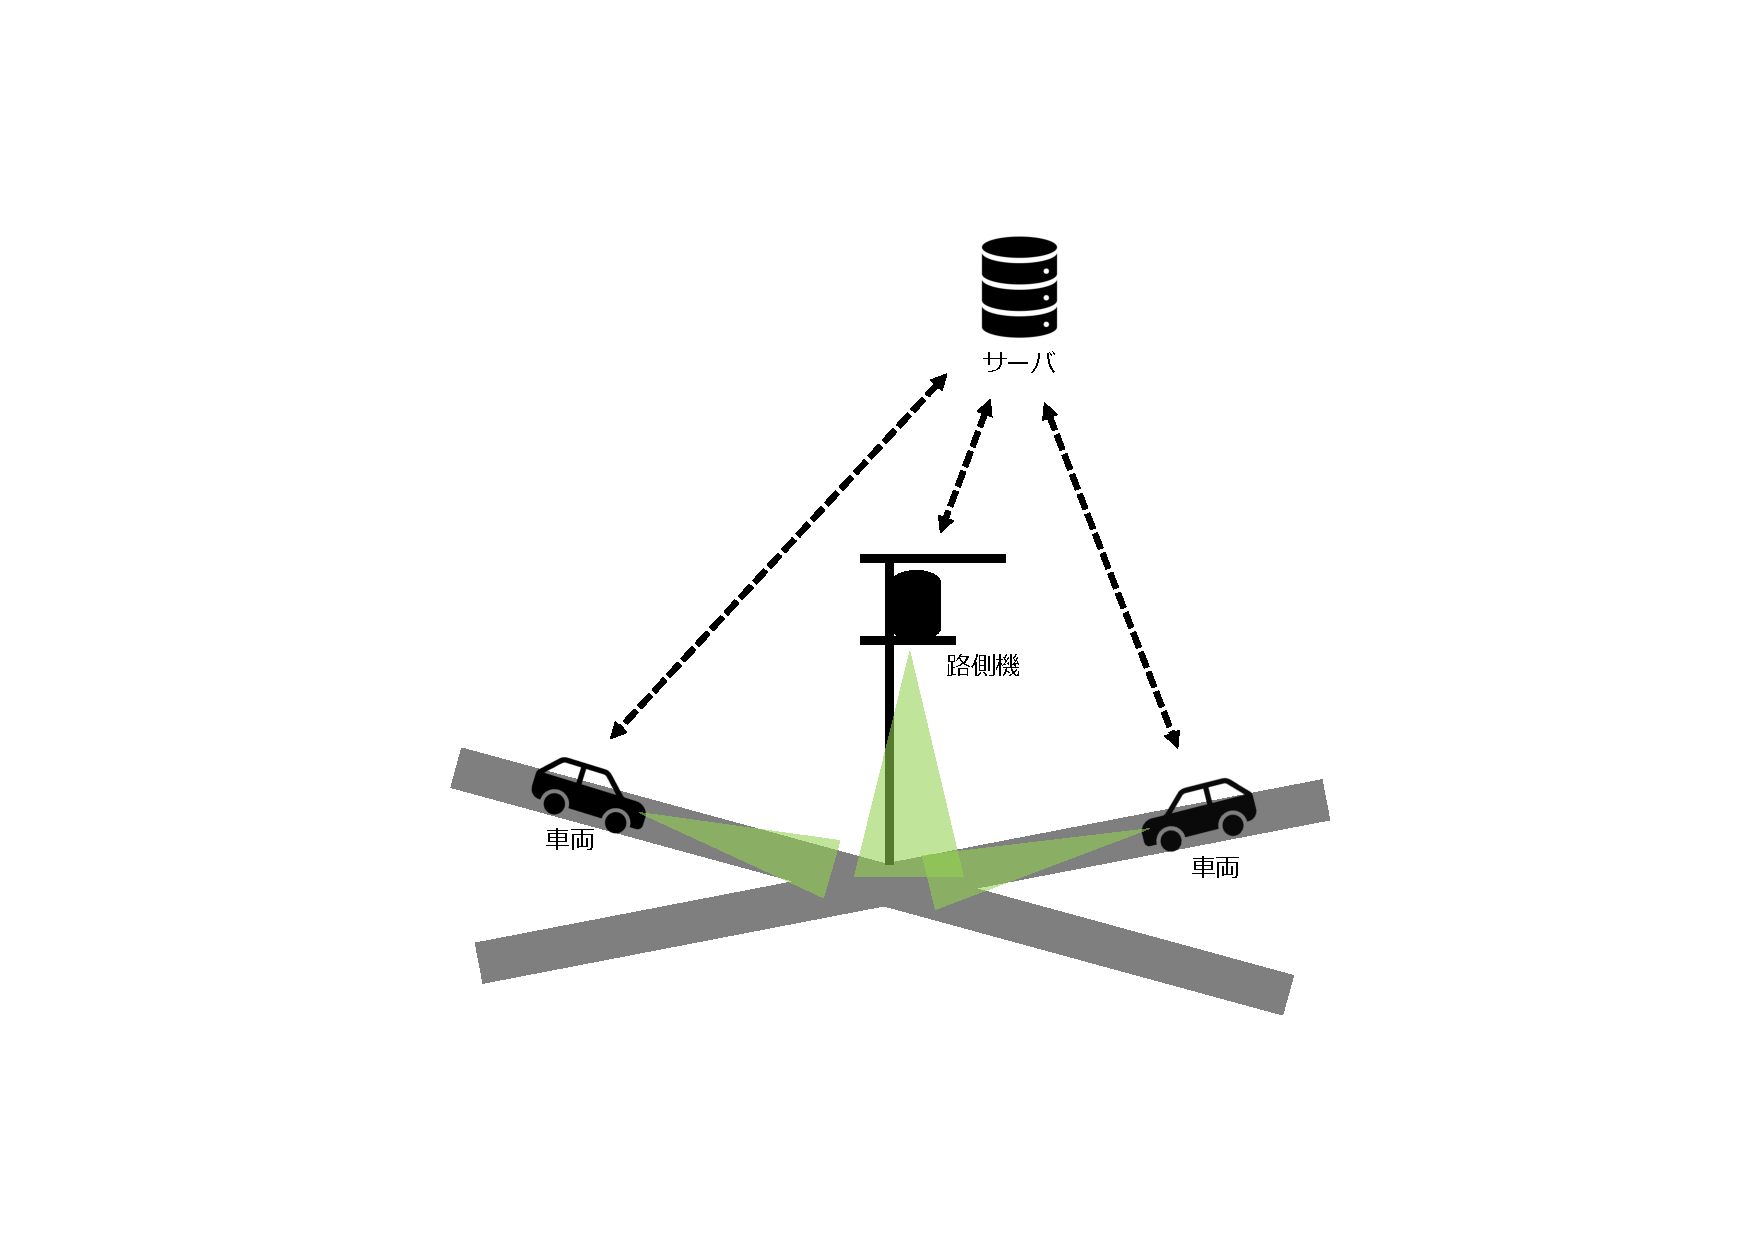
\includegraphics[width=\linewidth]{img/サーバを用いた協調型自動運転.pdf}
    \caption{サーバを用いた協調型自動運転}
    \label{fig:CAD}
  \end{figure}

\section{目的}
\label{sec:目的}

    本研究では,車両が集中した場合に通信のQoSが保証されず、そのことを車両が事前に判断することができない問題を解決するため,ネットワーク仮想化技術を利用して通信のQoSを予測し,車両の将来の通信のQoSを予約することを提案する.
    ネットワークシミュレーションを用いて通信モデルを構築し実験を行い,提案手法の有効性を評価する.

%アインシュタイン方程式は以下の通りである.\par

%\begin{equation}
%  R_{\mu\nu} - \frac{1}{2} g_{\mu\nu} R = \frac{8\pi G}{c^2} T_{\mu\nu}
%\end{equation}

%ベクトルの書き方は以下の通り.\par

%\begin{itemize}
%  \item 普通の$\alpha$は\verb|\alpha|で書く。
%  \item \verb|$\vec{\alpha}$| で $\vec{\alpha}$
%  \item \verb|\usepackage{bm}| している場合は
%        \verb|$\bm{\alpha}$| で $\bm{\alpha}$
%  \item 並べると,$\alpha$, $\vec{\alpha}$, $\bm{\alpha}$
%\end{itemize}

\section{本論文の構成}
\label{sec:本論文の構成}

  第\ref{chap:関連研究}章では,協調型自動運転のV2X通信のQoS予測を行った関連研究について述べる.
  第\ref{chap:提案手法}章では,ネットワーク仮想化技術を利用したV2X通信の制御と,QoSの予測および予約の方法について述べる.
  第\ref{chap:評価}章では,提案手法の有効性を評価するための実験方法とその評価結果について述べる.
  第\ref{chap:考察}章では,実験によって得られた結果に対して考察を行う.
  第\ref{chap:おわりに}章では,本論文のまとめを述べる.

%----------------------------------------------------------------------

\chapter{関連研究}
\label{chap:関連研究}

  協調型自動運転では,車両が周囲の車両や路側機、サーバなどとリアルタイムで情報を共有することで,安全かつ効率的な交通システムを構築することができる.
  車両による事故を防ぐなどのユースケースに対してV2X通信を行うため,協調型自動運転のための通信は厳しいQoSの要件が決められており,パケットロス率や通信遅延について詳細に要求されている\cite{5GAA}.
  しかし,V2X通信では車両の高い移動性や交差点における車両の集中など,様々な要因が通信のQoSに影響を与える\cite{cause}.
  QoSの急激な低下が発生した場合,協調型自動運転におけるアプリケーションの機能不全が発生し,状況によっては人間の安全を脅かす可能性がある\cite{danger}.
  そのため,QoSの予測は重要であり,QoSの変化を予測することで事前に必要な対策を講じることができる.\par
  Barmpounakisらは,5Gのネットワークからデータを収集・分析する機能を利用してQoSに関する指標を求め,地図情報をグリッドに分割してQoSの指標を用いてクラスタリングすることで,機械学習を用いてQoSを予測した\cite{AI}.
  ネットワークシミュレータを用いた実験により,クラスタの数と予測精度のトレードオフの関係を示した.
  また,Xuらは,深層学習モデルの1つであるTransformer\cite{Transformer}の長期時系列予測モデルであるInformer\cite{Informer}を利用し,V2X通信の時間的および局所的な特徴を考慮したQoS予測を行った\cite{Informer-based}.
  実際の交通渋滞を模倣した環境でV2X通信に関するデータを収集し,パケットロス率および通信遅延について予測精度の向上を示した.\par
  これらの研究を含めて,V2X通信のQoS予測に関する研究は機械学習を用いたものが多く見られる,V2X通信特有の拘束条件のもとに,複数の機械学習の比較や計算効率性の向上を目指している.
  機械学習を用いた予測では過去のデータから傾向をもとに予測を行うため,例えばある道路において通勤時間帯に車両が混雑するというデータがある場合,次の日もその時間帯に道路は混雑すると予測する.
  しかし,道路工事や交通事故などにより車両の走行ルートに変更が生じた場合,道路が混雑するエリアを正しく予測できない可能性がある.
  そのため,過去のデータだけではなく,現時点での車両の走行ルートなどの情報から,近い将来のQoSを予測することが重要である.
  また,車両は自身の情報およびサーバから受信する情報しか持たないため,他の車両の走行ルートなどからある地点でのQoSが保証されるかを予測することができない.
  したがって,QoS予測のもとに各車両のQoSが保証されるかを判別し,車両に通知する仕組みが必要となる.

%----------------------------------------------------------------------
\chapter{提案手法}
\label{chap:提案手法}

\section{ネットワーク仮想化技術を利用したネットワーク}
\label{sec:ネットワーク仮想化技術を利用したネットワーク}

\subsection{協調型自動運転のためのネットワーク}

協調型自動運転における車両とサーバの通信方式については様々な種類のものが議論・検討されているが,ここではセルラーネットワークを利用して基地局を介して通信する方式を考える.
車両は協調型自動運転を行うに際して,近くにある基地局を介してサーバと通信を行う.
サーバをどれほどの間隔で地理的に分散配置し,サーバ1台あたり何基の基地局と対応するかについても,基地局1基にサーバが1台とするなどの様々な議論があるが,本研究では複数の基地局に対して1台のサーバが対応するネットワークを考える.
サーバは自身が対応する基地局の通信範囲内を管轄するエリアとして,管轄エリア内の車両の協調型自動運転に関する通信や情報の処理を担当する.
% なお,章で述べたように,協調型自動運転ではクラウドサーバが複数のエッジサーバから定期的に情報を集約・処理することが検討されているが,本研究では車両とエッジサーバの通信のみを対象とし,クラウドサーバとの通信については考慮しない.

\subsection{ネットワーク仮想化技術による通信制御}
\label{ネットワーク仮想化技術による通信制御}

% 協調型自動運転において,サーバの管轄領域内に通信帯域で収容可能な台数以上の車両が集中した場合に,通信のQoSが保証されず,そのことを車両が事前に判断することができない事態が懸念される.
% そこで,本研究ではネットワーク仮想化技術を利用してQoSが保証されるかを予測し,予測結果を車両に通知することを考える.
通信のQoSを予測・予約するにあたり,車両と基地局,サーバの通信を制御するために,本研究ではネットワーク仮想化技術を利用する.
ネットワーク仮想化技術とは,ソフトウェアを介してネットワークを一元管理する技術である.
ネットワーク仮想化技術では,コントローラと呼ばれる機器がネットワークの状況の把握や経路の変更・更新を行うため,状況に合わせた柔軟なネットワークの変更が可能となる.
本研究では,\figref{fig:NV}に示すように複数のサーバとその管轄領域内の車両との通信を1台のコントローラが管理することを考える.
コントローラは,サーバと接続し,QoS予測に必要な情報を車両やサーバから受け取る.
その後、コントローラが\ref{sec:QoS予測}節で述べるQoS予測を行い,車両に対して\ref{sec:QoS予約}節で述べるQoS予約を行う.
なお,コントローラとサーバは有線で接続されており,通信遅延やパケットロスなどの影響は極めて小さいものとする.\par

\begin{figure}[tb]
  \centering
  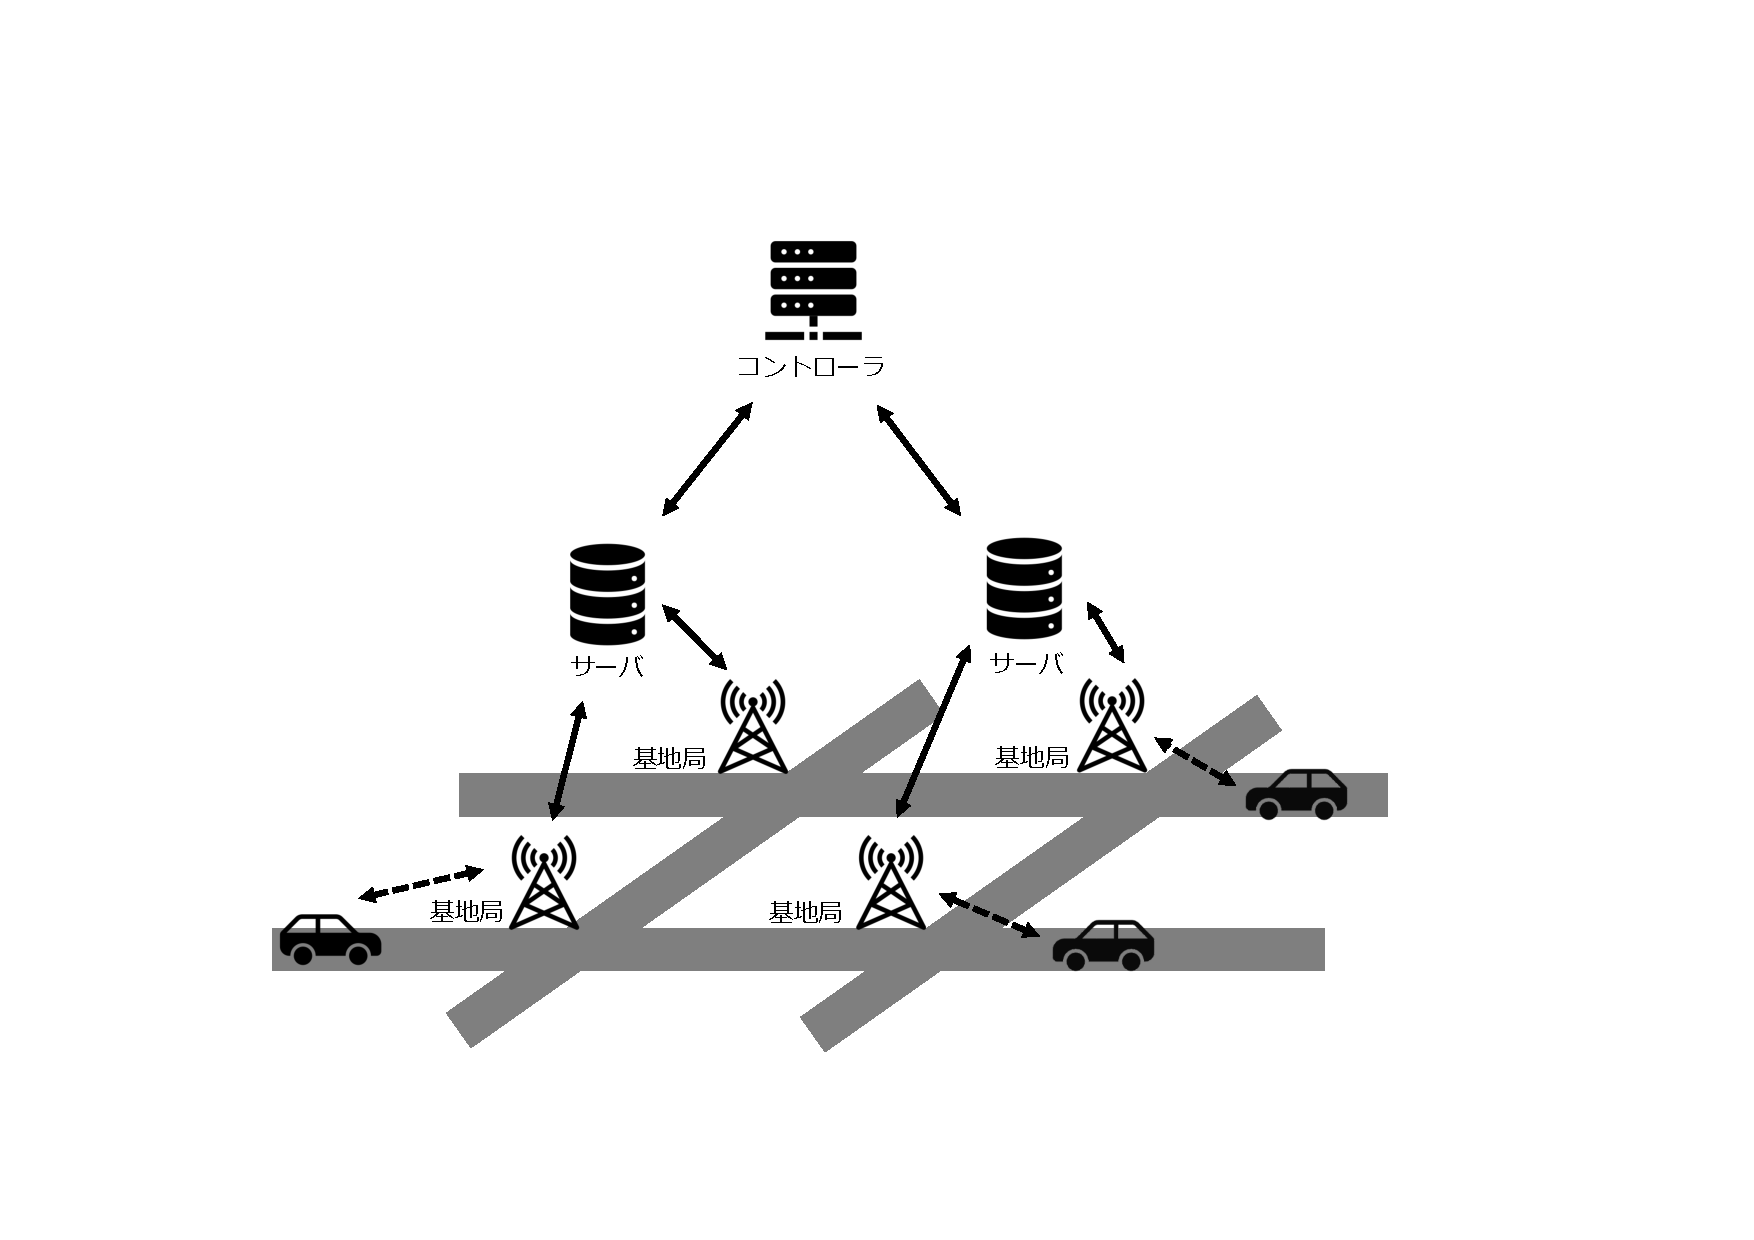
\includegraphics[width=\linewidth]{img/ネットワーク仮想化技術を利用したV2X通信の制御.pdf}
  \caption{ネットワーク仮想化技術を利用したV2X通信の制御}
  \label{fig:NV}
\end{figure}

ネットワーク仮想化技術を利用して通信制御を行うにあたり,コントローラは車両とサーバ間の通信帯域を\figref{fig:bandwidth}のように3つに分類する.

\begin{description}
  %\setlength{\leftskip}{5.5cm}
  \item[QoS予測・予約に必要な通信帯域]\mbox{}\\
    この通信帯域はコントローラがQoSを予測するのに必要な情報を車両から収集したり,QoSの予約を車両に通知したりするために用いられる.
    通信帯域が逼迫した際に,QoS予測・予約に必要な通信のQoSが保証できない場合,その次のQoSの予測や,車両がこれから到達する地点においてQoSが保証されるか否かの通知に障害が発生する可能性がある.
    そのため,この通信帯域は常に確保されているのとし,仮にサーバの管轄エリア内に物理的に限界な台数まで車両が集中したとしても,この通信帯域が全体の通信帯域を超えることはないように全体の通信帯域が設定されているものとする.
    この通信帯域で行われる通信の内容は時刻によって大きく変化するものではなく,1台あたりの通信量は大きく変化しないが,車両台数の増減に比例して通信量も変化する.
  \item [協調型自動運転のための通信帯域]\mbox{}\\
    この通信帯域は,協調型自動運転を行うため,車両が自身の走行情報や自車両に搭載されたセンサで認識した情報等をサーバに送信したり,サーバが複数の車両や路側機から収集・統合した情報を車両に送信したりする際に用いられる.
    この通信帯域で行われる通信の通信量は,車両の運転操作や周囲の走行環境等によって変化し,その通信量はQoS予測・予約のための通信と比較して通信量が大きいため,サーバの管轄領域内に車両が集中することにより,通信帯域が逼迫する恐れがある.
    したがって,本研究ではこの通信帯域を対象としてQoSの予測・予約を行う.
  \item [常に確保しておく余剰の通信帯域]\mbox{}\\
    この通信帯域は,通信量の変動やQoS予測の誤差を吸収するために,常に一定分確保されている通信帯域である.
    車両台数等によって変動することはなく,他の2つの通信帯域と比較してそれほど大きな通信帯域ではない.
    QoS予測・予約においては使用可能な通信帯域から除外して考える.
\end{description}

  \begin{figure}[tb]
    \centering
    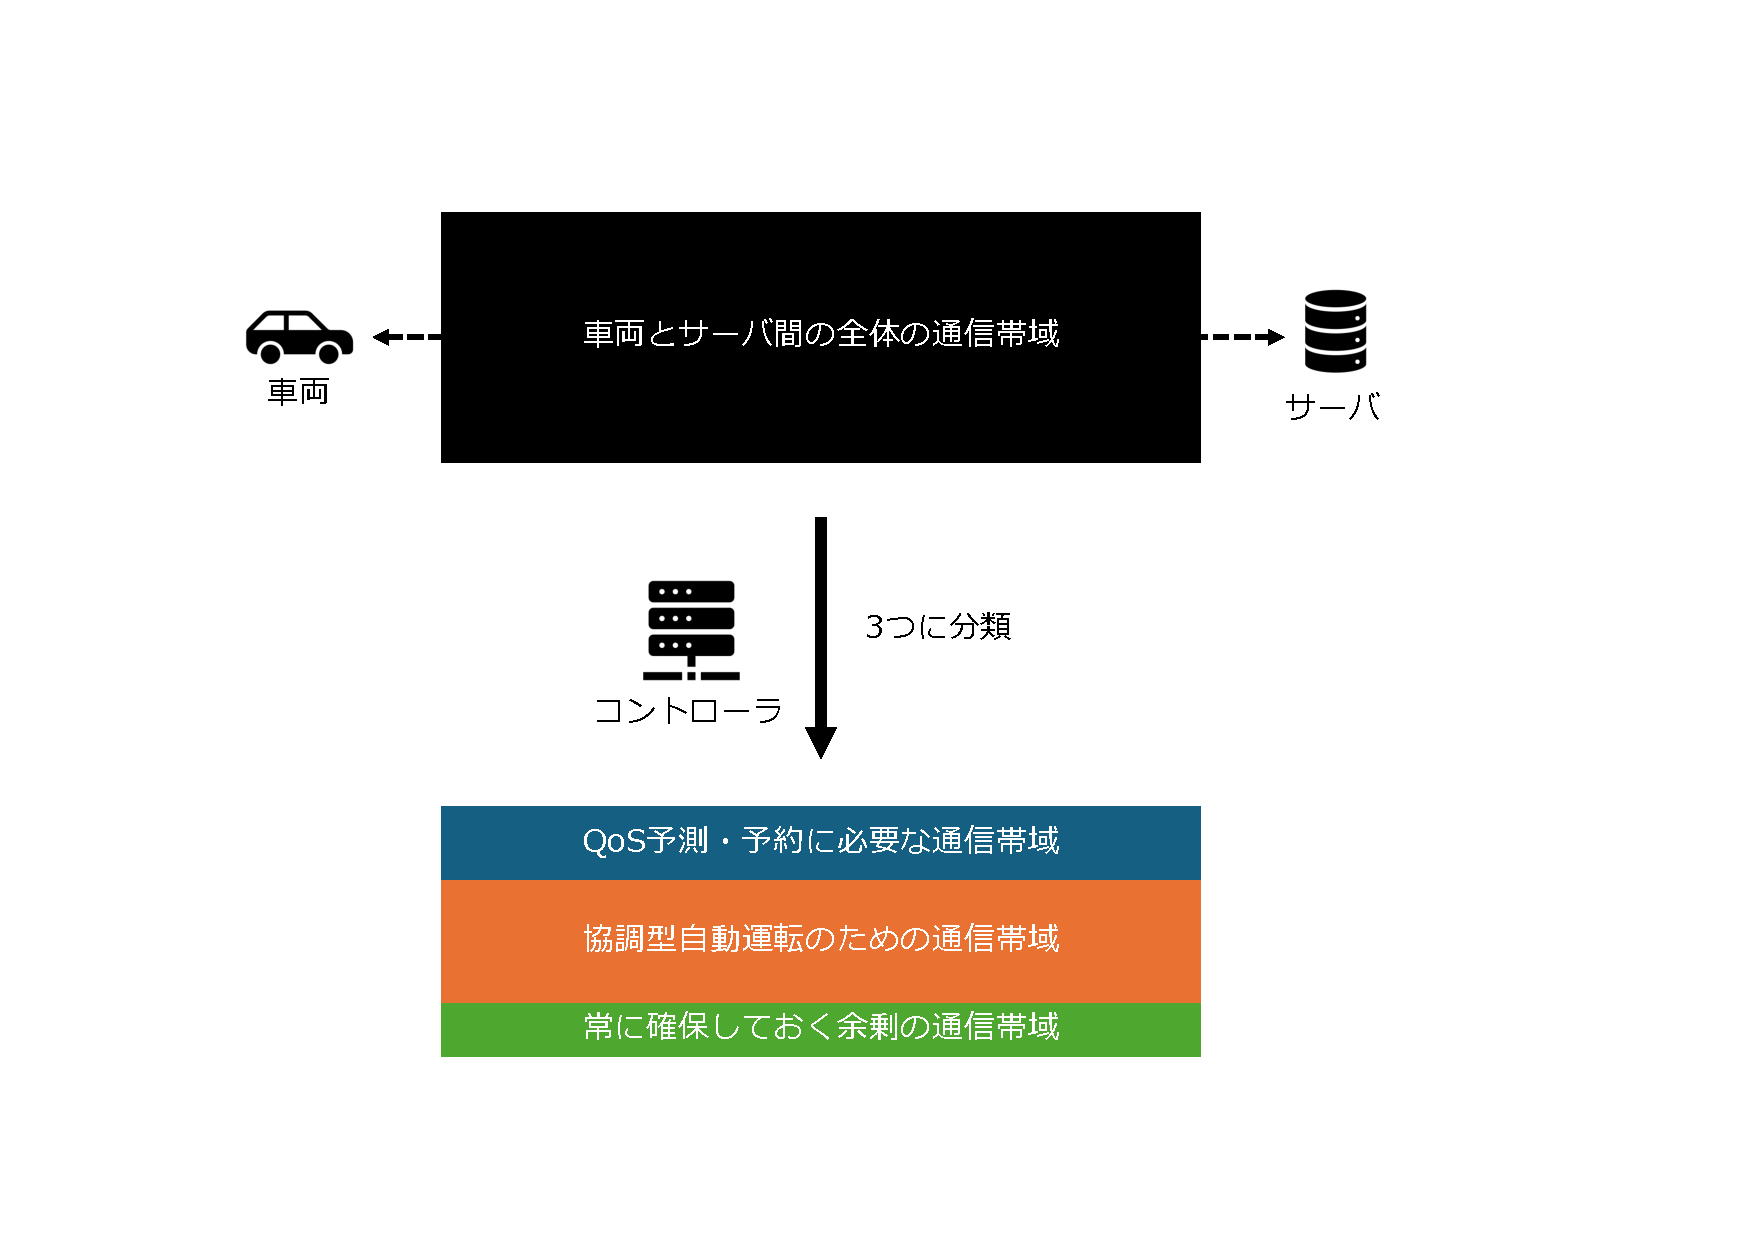
\includegraphics[width=\linewidth]{img/コントローラによる通信帯域の分類2.pdf}
    \caption{コントローラによる通信帯域の分類}
    \label{fig:bandwidth}
  \end{figure}

\section{QoS予測}
\label{sec:QoS予測}

\subsection{コントローラが管理する情報}

サーバの管轄エリア内に車両が集中した場合,協調型自動運転のための通信の通信量が増大し,通信帯域が逼迫する恐れがある.
したがって,協調型自動運転のための通信のQoSを予測するためには,コントローラは一定時刻後のサーバの管轄エリア内の車両の集中状況および使用される通信帯域を予測する必要がある.
そのために,コントローラは以下の情報を保持している.

\begin{itemize}
\item コントローラの管轄エリアの地図情報
\item コントローラが管轄するサーバおよび基地局の位置
\item コントローラが管轄する各サーバにおいて使用できる最大の通信帯域
\item \ref{sec:QoS予約}節で述べるQoS予約によってすでに確保されている通信帯域
\end{itemize}

また,コントローラは車両から以下の情報を定期的に受け取る.

\begin{itemize}
\item 車両を一意に識別可能なID(車両ID)
\item 走行計画
\end{itemize}

以上の情報を用いて,コントローラは一定時刻後の通信のQoSを予測する.

\subsection{QoSの予測方法}
\label{QoSの予測方法}

協調型自動運転のための通信のQoSが保証されるかは,一定時刻後に使用される予定の通信量の合計を求め,使用できる最大の通信帯域と比較することで予測することができる.
一定時刻後に使用される予定の通信量の合計を求めるために,一定時刻後の車両の運転操作および集中状況を考える.
QoS予測の手順を\figref{fig:QoSPrediction}に示す.
コントローラは車両から定期的に受け取る走行計画から,一定時刻後の車両の予測位置を把握することができる.
ここで,一定時刻後のあるサーバの管轄エリア内の予測車両台数を$N$,1台あたりのQoS予測に必要な通信帯域を$B_{pred}$とすると,QoS予測に必要な通信帯域は

\begin{equation}
N * B_{pred}
\end{equation}

で求められる.
また,QoSの保証および予約は連続的に行われるため,一定時刻後の通信帯域において,それよりも前の時刻にすでにQoSが保証されている,すなわち通信帯域の一部が確保されている場合がある.
したがって,すでに確保されている通信帯域を$B_{saved}$,利用できる最大の通信帯域を$B_{max}$とすると,一定時刻後に利用可能な通信帯域は

\begin{equation}
B_{max} - (N * B_{pred} + B_{saved})
\end{equation}

となる.
$N$台全ての車両が協調型自動運転のための通信を行った場合に,この通信帯域で逼迫することがないかを予測することで,QoSを予測することができる.
協調型自動運転のための通信で使用する通信帯域は,車両の運転操作や周囲の走行環境や運転操作によって異なる.
ある車両の協調型自動運転における使用予測通信帯域を$B_{CAD}$とすると,

\begin{equation}
\sum_{k=1}^{n} B_{CAD_k} > B_{max} - (N * B_{pred} + B_{saved})
\end{equation}

である時に,$N$台全ての車両の通信のQoSを保証することはできないと予測される.
なお,使用予測通信帯域はあくまで予測されたものであり,多少の誤差を含む可能性があるため,\ref{ネットワーク仮想化技術による通信制御}項で述べたように

\begin{equation}
\sum_{k=1}^{n} B_{CAD_k} > B_{max} - \{(N * B_{pred} + B_{saved}) + B_{extra}\}
\end{equation}

のように誤差を吸収できる余分な通信帯域$B_{extra}$を考慮して計算するべきである.

\begin{figure}[tb]
  \centering
  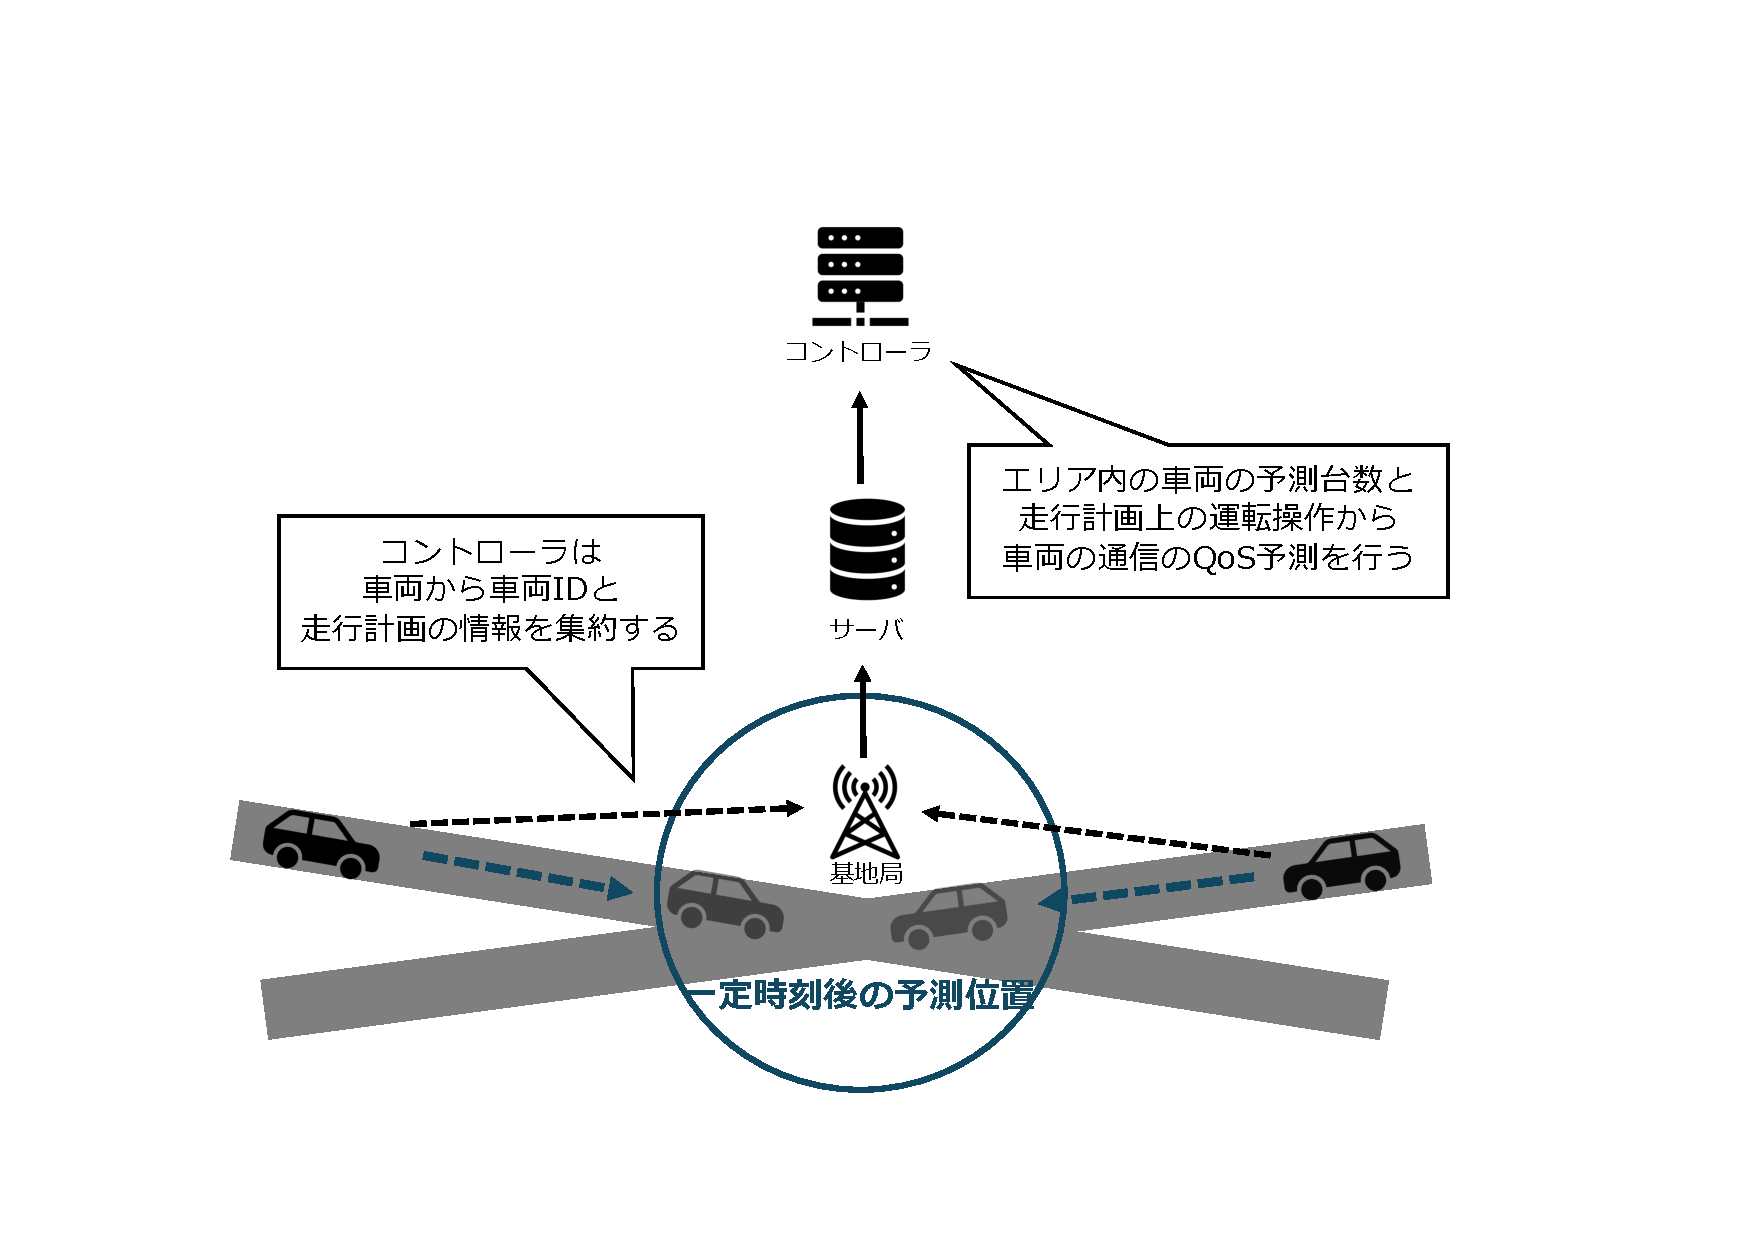
\includegraphics[width=\linewidth]{img/QoS予測の手順.pdf}
  \caption{QoS予測の手順}
  \label{fig:QoSPrediction}
\end{figure}

\section{QoS予約}
\label{sec:QoS予約}

\subsection{QoSの予約方法}

通信帯域が逼迫し,通信のQoSが保証されないことを車両が事前に判断できない場合,車両は通常時と同様に通信を試みるが,必要な情報を協調型自動運転で許容される時間内に受け取ることができないため,自車両が持つ情報のみで運転操作を行わなければならず,安全や効率の点で重大な問題となる.
そこで,本研究では,\figref{fig:QoSReservation}に示すように,QoS予測の結果をもとに,一定時刻後における通信帯域を車両ごとに確保するとともに,QoSが保証されるか否かを車両に通知する.
その時刻において協調型自動運転のための通信を行う車両を事前に決定することで,車両が集中した場合であっても通信帯域の逼迫を防ぐことができる.\par
まず,QoS予測の結果,

\begin{equation}
\sum_{k=1}^{n} B_{CAD_k} \leq B_{max} - \{(N * B_{pred} + B_{saved}) + B_{extra}\}
\end{equation}

となった場合,すなわち,全ての車両に対して一定時刻後の通信のQoSを保証することができると予測した場合を考える.
この場合,コントローラは一定時刻後の全ての車両の通信の帯域を確保し,車両IDをもとに該当する車両に対して一定時刻後の通信のQoSが保証されることを通知する.
これにより,全ての車両は問題なく協調型自動運転のための通信を行うことができる.\par
次に,

\begin{equation}
\sum_{k=1}^{n} B_{CAD_k} > B_{max} - \{(N * B_{pred} + B_{saved}) + B_{extra}\}
\end{equation}

となった場合,すなわち,全ての車両が通信を行った場合に通信帯域が逼迫し,通信のQoSが保証できないと予測した場合を考える.
この場合,全ての車両が通信を行った際に,通信帯域の逼迫により全ての車両が協調型自動運転の許容時間内に情報が受け取れない可能性があるため,通信帯域が逼迫しないように一部の車両を選択してQoSを保証し,残りの車両には通信を行わないよう通知することで通信帯域の逼迫を防ぐ.
QoSを保証する車両の選択は,一定時刻後における車両の運転操作の優先度を考慮して決定する.
例えば,一定時刻後において,他車両と調停しながら右左折を行なっている最中である車両と,特に前後の時刻と変わらず直進を続けている車両がいた場合,右左折を行なっている車両の通信のQoSを優先的に保証する.
優先度による車両の選択の後,同じ優先度から車両を選択しなければいけない場合はランダムに選択する.
しかし,本研究では検討の対象外としたが,QoSが保証されない車両も安全かつ効率的な運転のために,迂回経路の使用やその他の通信の併用などの方法で対策が必要であり,同じ優先度から選択する場合はそういった対策との兼ね合いを考慮して選択するのが望ましいと考えられる.

  \begin{figure}[tb]
    \centering
    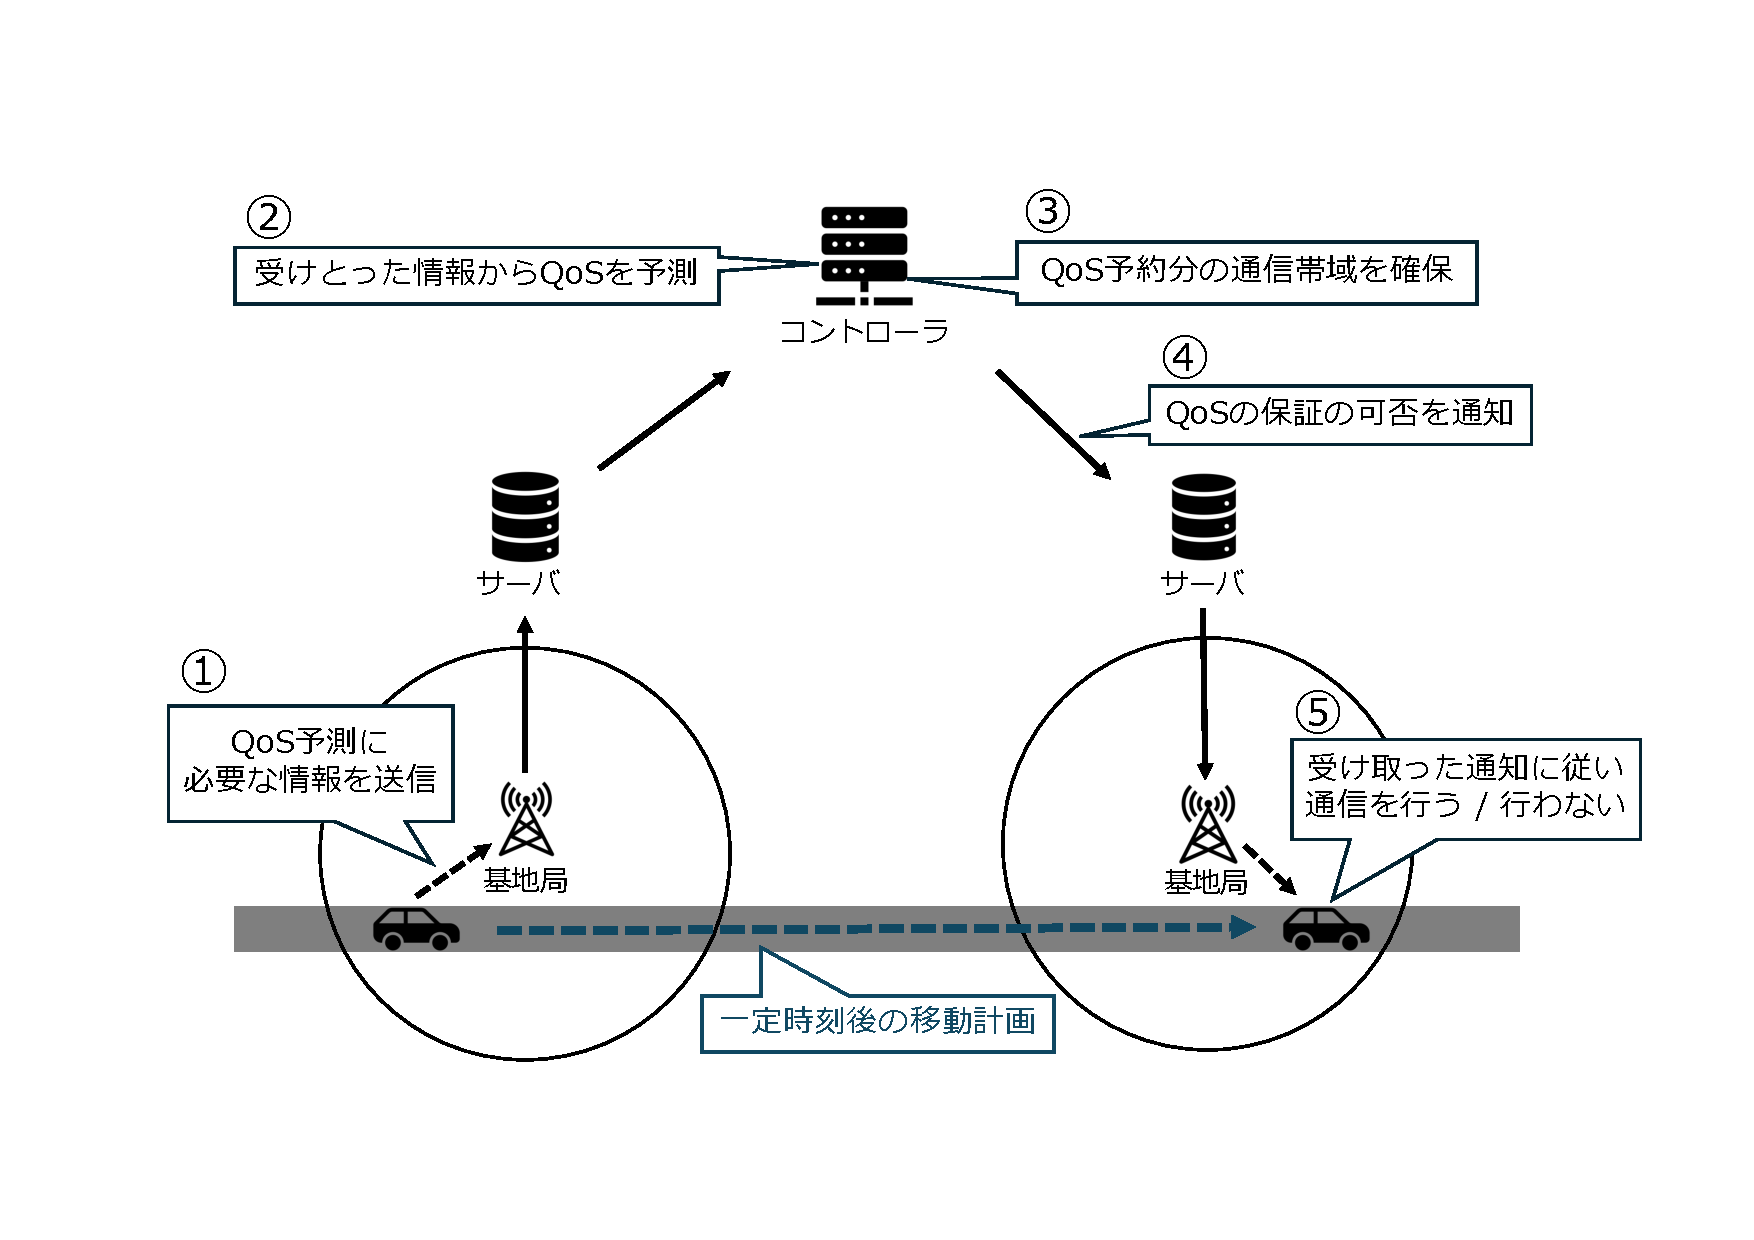
\includegraphics[width=\linewidth]{img/QoS予測・予約の手順.pdf}
    \caption{QoS予測・予約の手順}
    \label{fig:QoSReservation}
  \end{figure}

\subsection{QoSの予約時間}

\figref{fig:TurnRight}に示すように,一定時刻後に交差点を右折する車両の通信のQoSを保証する場合を考える.
この時,一定時刻ごとに新たにQoSを保証する車両を選択しているとすると,右折開始時にはQoSが保証されていたにもかかわらず,右折途中の新たなQoS予約でQoSが保証されなくなる,といった事態が発生する可能性がある.
右折などの周囲の車両と調停を必要とする運転操作や,自車両のセンサのみでは認識できない走行環境の認識を必要とする運転操作を行なっている最中に協調型自動運転のための通信を行えないと通知された場合,突然情報が遮断されることになるため,安全性に重大な問題が生じる.
そのため,QoSを予約する際に,コントローラは車両から受け取った走行計画から一定時刻後の運転操作を把握し,必要に応じてあらかじめそこから一定時間の通信帯域もまとめて予約しておく.
これにより,協調型自動運転のための通信の優先度が高い運転操作は,開始前に通信のQoSが保証されると通知されれば,その運転操作が完了するまで通信のQoSは保証されることになる.
QoS予約された通信帯域は,\ref{QoSの予測方法}項の$B_{saved}$としてSDNコントローラが保持し,以降のQoS予測の際に使用可能な通信帯域から除いて計算する.
運転操作が完了すると,車両はそのことをコントローラに通知し,通知を受け取ったコントローラは予約していた通信帯域を解放し,使用可能な通信帯域として計算する.

  \begin{figure}[tb]
    \centering
    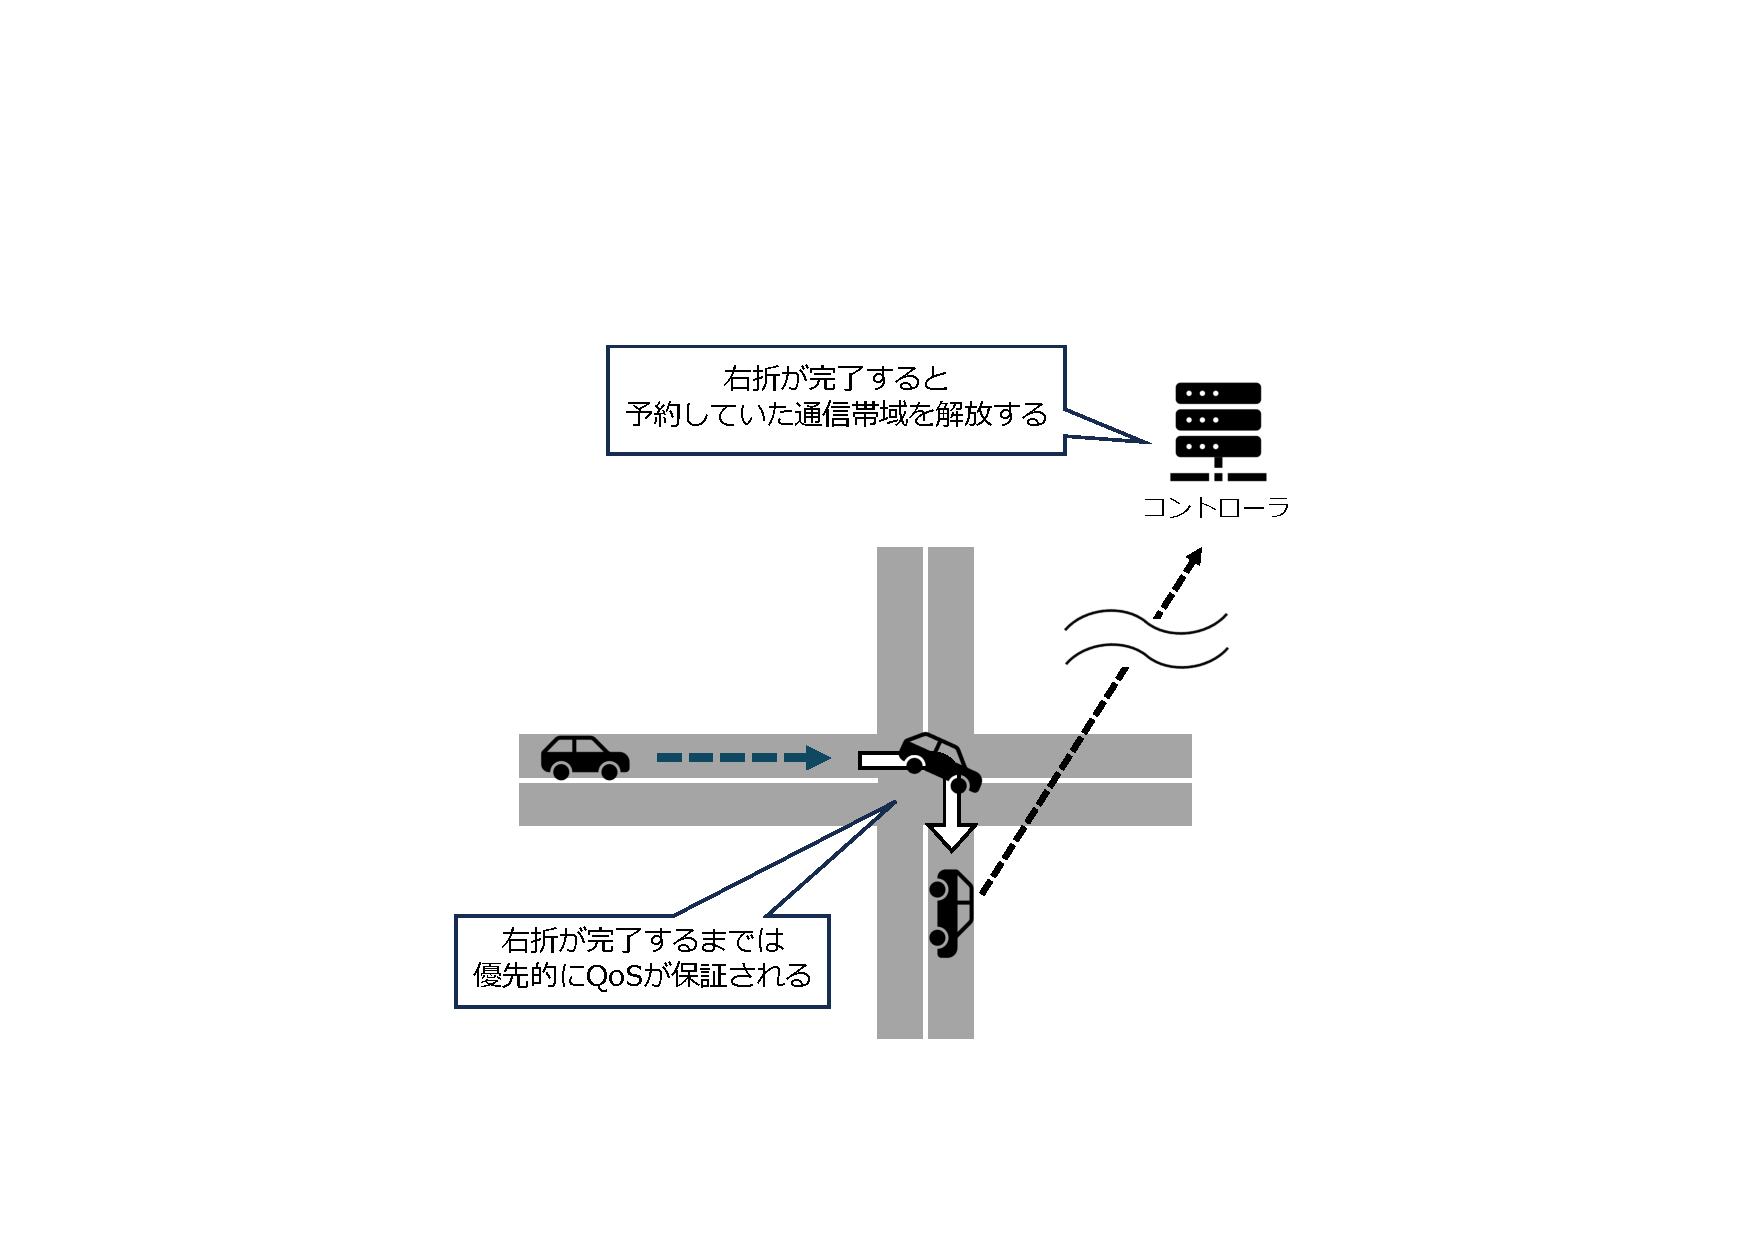
\includegraphics[width=\linewidth]{img/右折時のQoS予約2.pdf}
    \caption{右折時のQoS予約}
    \label{fig:TurnRight}
  \end{figure}

%\section{文献の引用の仕方}
%\label{sec:分権の引用の仕方}

%この文献\cite{LaTexWiki,渡辺豊2016}を参考にした.\par

%\section{図の挿入の仕方}
%\label{sec:図の挿入の仕方}

%図は以下のように挿入し,\figref{fig:sample1}と引用します.\par

%\begin{figure}[!tb]
%  \centering
%  
\includegraphics[width=\linewidth]{img/sample1.pdf}
%  \caption{サンプル画像1}
%  \label{fig:sample1}
%\end{figure}

%----------------------------------------------------------------------

\chapter{評価}
\label{chap:評価}

\section{評価環境}
\label{評価環境}

  提案したQoS予測・予約を適用することで,通信性能にどのような影響を与えるかを検証するため,ネットワークシミュレータであるns-3\cite{ns-3}を用いてシミュレーションによる評価を行った.
  \figref{fig:model}に示すようなネットワークモデルを構築し,サーバから車両に対して協調型自動運転のための通信のシミュレーションを行った.
  シミュレーションはQoS予測・予約を行わない場合と行う場合のそれぞれを行い,車両台数を変化させて通信性能を比較することでQoS予測・予約の有効性を評価した.\par

  \begin{figure}[tb]
    \centering
    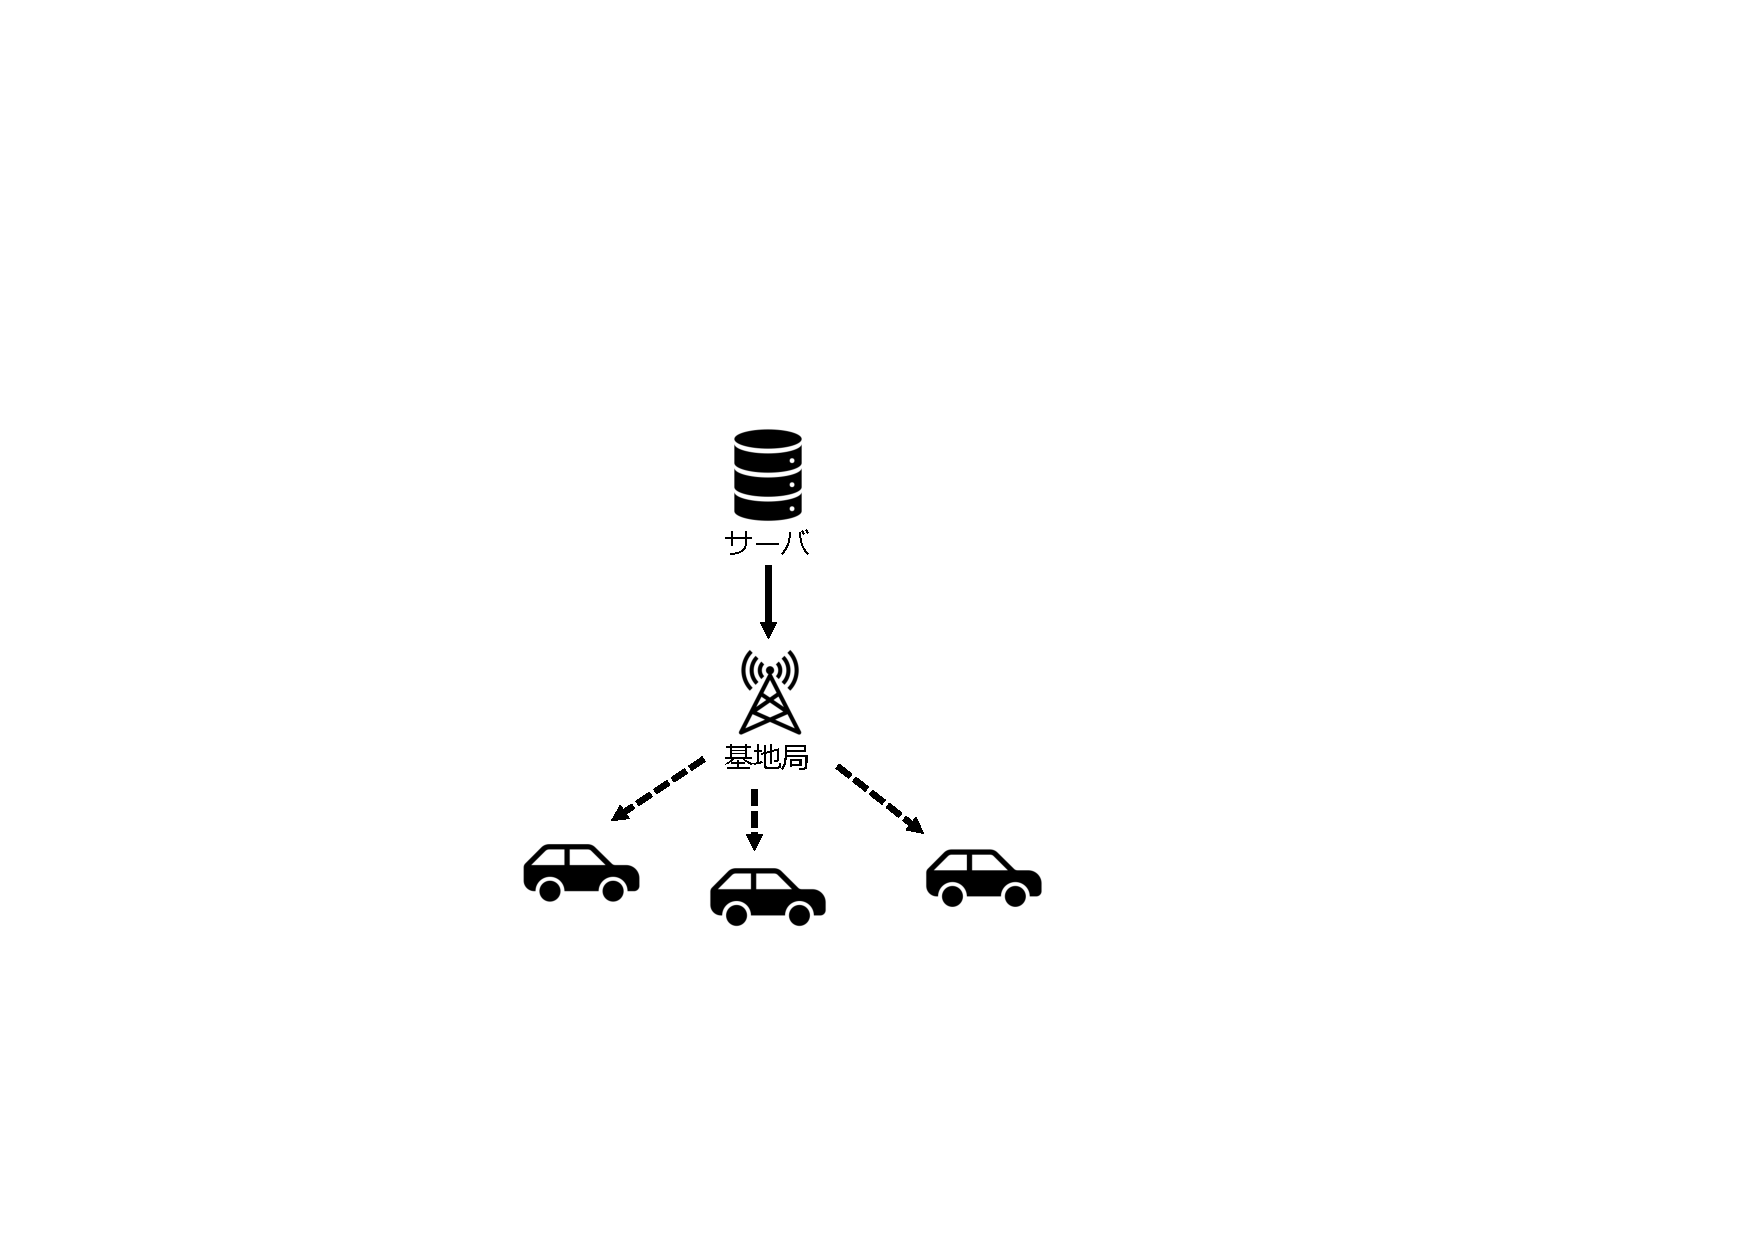
\includegraphics[width=0.41\linewidth]{img/シミュレーションモデル2.pdf}
    \caption{シミュレーションモデル}
    \label{fig:model}
  \end{figure}

  QoS予測・予約を行わない場合は,通信帯域が逼迫しているか否かに関わらず,サーバから車両に対して協調型自動運転のための通信を試み続ける.
  一方で,QoS予測・予約を行う場合は,QoS予測・予約によって通信帯域が確保される車両をあらかじめ計算し,その台数の車両に対してのみ協調型自動運転のための通信を行う.
  QoS予測・予約にも通信帯域を消費するため,QoS予測・予約を行う場合は,QoS予測・予約に必要な通信帯域を車両台数より計算し,行わない場合の使用可能な通信帯域からその分を差し引いたものを使用可能な通信帯域とする.
  QoSが保証される車両台数の計算やQoS予測・予約に必要な通信帯域は\tabref{tab:parameter}に示す評価パラメータより計算する.\par
  
  \begin{table}[tb]
    \centering
    \caption{評価パラメータ}
    \label{tab:parameter}
    \begin{tabular}{cc}
      \hline
      仮想環境 & VirtualBox7.0.8\\
      OS & Ubuntu22.04\\
      シミュレータ & NS3 5g-lena NR Module\\
      下り速度 & 100Mbps\\
      パケットサイズ & 1000byte\\
      送信間隔 & 100ms\\
      1台あたりのQoS予測に必要な通信帯域 & 10Kbps\\
      \hline
    \end{tabular}
  \end{table}

  協調型自動運転のための通信の性能を評価するため,協調型自動運転のための通信について,サーバから車両までの通信遅延およびパケットロス率を測定する.
  QoS予測・予約を行わない場合は全ての車両に対する通信遅延およびパケットロス率の平均を求める.
  QoS予測・予約を行う場合は,QoSが保証された車両に対する通信遅延およびパケットロス率の平均を求め,QoS予測・予約を行わない場合と比較する.


\section{評価結果}
\label{sec:評価結果}

\subsection{通信遅延}

  QoS予測・予約を行わなかった場合と行った場合の通信遅延の比較をに示す.


\subsection{パケットロス率}

  QoS予測・予約を行わなかった場合と行った場合のパケットロス率の比較をに示す.


%   \begin{figure}[tb]
%     \centering
%     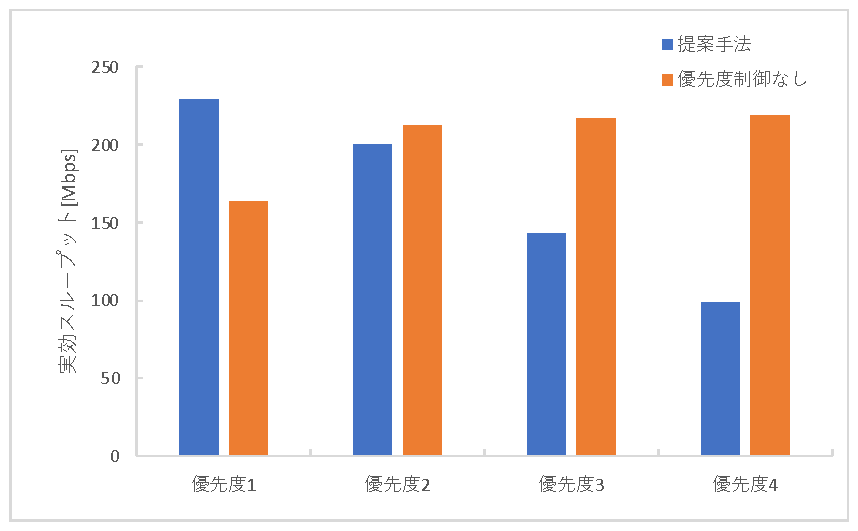
\includegraphics[width=0.85\linewidth]{img/throughput_1.pdf}
%     \caption{優先度制御しない場合とのスループットの比較}
%     \label{fig:throughput_1}
%   \end{figure}


%   \begin{figure}[tb]
%     \centering
%     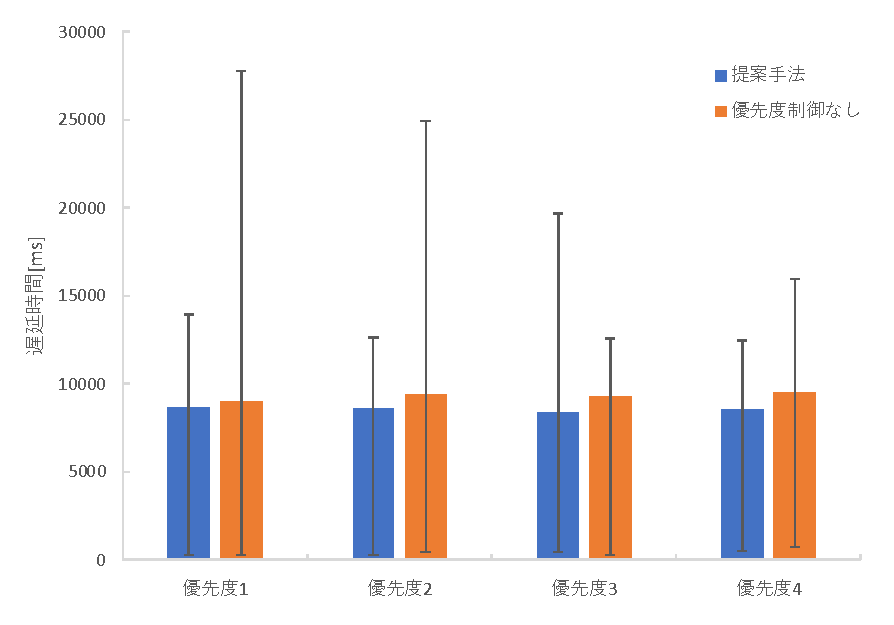
\includegraphics[width=0.85\linewidth]{img/RTT_1.pdf}
%     \caption{優先度制御しない場合との遅延時間の比較}
%     \label{fig:RTT_1}
%   \end{figure}


%   \begin{figure}[tb]
%     \centering
%     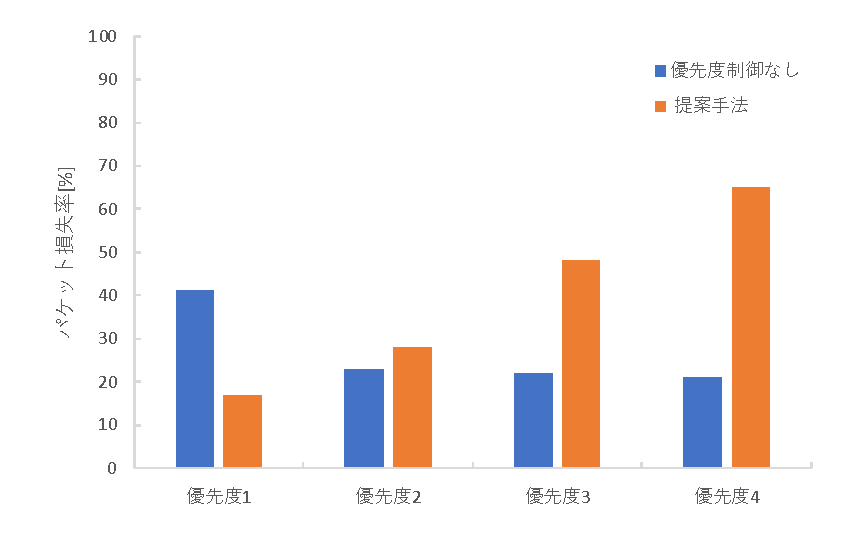
\includegraphics[width=0.85\linewidth]{img/packetloss_1.pdf}
%     \caption{優先度制御しない場合とのパケット損失率の比較}
%     \label{fig:packetloss_1}
%   \end{figure}

%----------------------------------------------------------------------

\chapter{考察}
\label{chap:考察}

  本章では,\ref{chap:評価}章で述べた結果をもとに提案手法の有効性を考察する.
  提案手法を用いることで,優先度制御を行わない場合や固定された優先度分類を用いた場合と比較して,スループット,遅延時間,パケット損失率に与える影響を考察する.\par

  まず,\ref{sec:通信性能}節の結果をもとに,優先度制御を行わない場合と比較して,提案手法の有効性を考察する.
  \figref{fig:throughput_1}に示すように,最も優先度の高い優先度1の通信のスループットは,提案手法を用いた場合の方が優先度制御しない場合と比較して向上している.
  しかし,優先度2\textasciitilde4の通信ではスループットが低下しており,通信全体のスループットは低下している.
  また,\figref{fig:packetloss_1}に示すように,優先度1の通信のパケット損失率は改善してるが,優先度2\textasciitilde4の通信のパケット損失率は増加した.
  これは,提案手法では各ポートに設定した通信量の閾値を超えた際にアドミッション制御を行うため,まだ通信帯域が逼迫しきっておらず,パケットを送信する余裕があったがパケットを破棄してしまったことが原因である.
  一方,優先度制御を用いない場合は,通信帯域の限界のみでしかパケットの損失が発生しないため,提案手法を用いた場合と比較して通信全体のスループットとパケット損失率は高い品質を示した.
  アドミッション制御を,通信量の閾値をもとに行うのではなく,通信帯域の逼迫率をもとに行うことで,スループットとパケット損失率の改善が可能である.\par

  \figref{fig:RTT_1}に示すように,デバイスがパケットを送信してからその応答がデバイスに返ってくるまでの遅延時間は,提案手法を用いた場合が優先度制御しない場合と比較して軽減した.
  これは,優先度制御を用いない場合では,通信帯域が逼迫した際にTCPの確認応答と再送制御が行われるため遅延時間が増加するのに対して,提案手法では通信量が閾値を超えた場合にパケットが破棄されるため,確認応答と再送制御がそもそも行われず,その分遅延時間が軽減されることが原因である.
  通信帯域の逼迫率を監視し,パケットの到達が見込めない時はパケットを破棄することで,遅延時間を軽減することが可能である.\par

  次に,\ref{sec:動的な優先度分類}節の結果をもとに,提案手法の動的な優先度分類の有効性を考察する.
  \figref{fig:throughput_2}に示すように,提案手法を用いた場合では優先度の変更に合わせてアドミッション制御を行なったため,カテゴリ4=優先度3のスループットがカテゴリ3=優先度4のスループットよりも高くなっている.
  一方,固定された優先度分類では,カテゴリ4=優先度3のスループットがカテゴリ3=優先度4のスループットよりも低くなっており,優先度の変化に対応できていない.
  また,パケット損失率についても,提案手法ではカテゴリ4=優先度3のパケット損失率がカテゴリ3=優先度4のパケット損失率よりも低下しているのに対して,固定した優先度分類ではカテゴリ4=優先度3のパケット損失率がカテゴリ3=優先度4のパケット損失率より高くなっている.
  動的な優先度分類によって,優先度の変更に対応した優先度制御を実現した.\par

  

%----------------------------------------------------------------------
% おわりに
%----------------------------------------------------------------------
\chapter{おわりに}
\label{chap:おわりに}

%まとめを書きましょう.800字から1000字ぐらいでまとめてください.背景,解決すべき問題点,提案内容,結果,考察,研究の意義などを含めて記載してください.結果については,過去形(・・・実施した.・・・評価した.・・・確認した.など)で記載してください.

  自車両の車載センサのみで認識できる範囲は限定的であるため,他の車両や路側機のセンサの情報をサーバを利用して共有することで安全かつ効率的な走行を目指す協調型自動運転の研究がおこわれている.
  協調型自動運転に用いられるサーバは,処理負荷の分散や通信遅延の軽減のために地理的に分散配置されており,そのサーバの管轄するエリア内にいる車両や路側機の情報を集約・統合する.
  しかし,サーバまでの通信帯域は限られている場合が多く,車両が管轄エリア内に集中した場合に通信帯域が逼迫する恐れがある.
  協調型自動運転では低遅延での通信が求められるが,通信帯域が逼迫すると,許容される遅延時間内に情報を受け取ることができず,通信のQoSが保証されない.
  また,車両は事前に通信のQoSが保証されるか否かを把握することができないままに協調型自動運転を試みることになるため,安全性や効率の点で重大な問題となる.\par
  本研究では,ネットワーク仮想化技術を利用したQoS予測・予約を行った.
  ネットワーク仮想化技術を利用することで,QoS予測に必要な情報の集約と,QoS予約に必要な通知を行った.
  コントローラは集約した情報から,ある時刻でのサーバの管轄エリア内の車両台数と車両の運転操作を計算し,必要となる通信帯域を予測した.
  保持する情報から使用可能な通信帯域を計算し,必要となる通信帯域と比較することでQoSを予測した.
  また,QoS予測の結果から,QoSを保証する車両を決定し,車両に通知することでQoSを予約した.
  使用可能な通信帯域が十分にある場合は全ての車両に対してQoSを予約し,通信帯域が十分にない場合は車両のその時刻での運転操作から通信帯域が確保されるべき優先度を考慮し,QoSを予約する車両を決定した.\par
  サーバから車両へと情報を送信する通信モデルを構築し,ネットワークシミュレーションを行うことで提案手法の有効性を検証した.

%----------------------------------------------------------------------
% 謝辞
%----------------------------------------------------------------------
% サンプル
% 本研究を進めるにあたって,多大なご指導とご支援を賜りました同志社大学理工学部の佐藤健哉教授に心より感謝致します.また,3年間研究生活を共に過ごし,研究に就職活動と共に乗り越えたネットワーク情報システム研究室の同期,研究・就職活動の相談に乗ってくださった先輩,研究室生活で慕ってくれた後輩,さらに様々な場面で支えてくれた家族と友人へ感謝します.
%----------------------------------------------------------------------
\chapter*{謝辞}
\addcontentsline{toc}{chapter}{謝辞}  % 章番号のない章を目次に表示させる
\label{sec:Acknowledgments}
%謝辞には章番号をつけなくてもよいので,\verb|\chapter*{}| という具合に書きます.

  \noindent
  本研究を進めるにあたって,多大なご指導とご支援を賜りました同志社大学理工学部の佐藤健哉教授に心より感謝いたします.
  また,研究内容について親身にアドバイスをくださった山本浩太郎先輩をはじめとしたネットワーク情報システム研究室のみなさまには,大変お世話になりました.
  さらに,学校生活や研究活動を支えて支えてくれた友人と家族へ感謝いたします.

%----------------------------------------------------------------------
% 付録
%----------------------------------------------------------------------
%\appendix
%\chapter{ソースコード}
%\label{apndx:src}

%プログラム文とかを書きたい場合は,以下のようにしてみます.\verb|\usepackage{ascmac}|して\verb|screen| 環境を使うと,枠がつきます.

%\begin{screen}\begin{verbatim}
%#include <iostream>
%using namespace std;

%int main() {
%  for(int i = 1; i <= 5; i++) {
%    cout << "こんにちは, C++ の世界! " << i << endl;
%  }
%  return 0;
%}
%\end{verbatim}\end{screen}

%----------------------------------------------------------------------
% 参考文献
%----------------------------------------------------------------------
\renewcommand{\bibname}{参考文献}

% thebibliography を利用する場合は以下を使用(拘りがなければこちらでOK)
\begin{thebibliography}{99}
  \bibitem{AD}
  横山俊夫, 波多野邦道, 小沢浩一郎, 樋山智, 小高賢二, 自動車業界における自動運転実用化に向けた取り組み, 学術の動向, Vol.25, No.5, pp.17-21 (2020).

  \bibitem{CAD}
  辰巳周一, 樋口竜貴, 染谷竜太, 協調型自動運転の実現に向けた最新の技術動向と課題, 電気学会誌, Vol.140, No.5, pp.308-311 (2020).

  \bibitem{ITS}
  菅沼英明, ITS・自動運転の動向と今後, 電子情報通信学会 通信ソサイエティマガジン, Vol.15, No.2, pp.102-108 (2021).

  \bibitem{edge}
  Fuhui Zhou, Rose Qingyang Hu, Zan Li and Yuhao Wang, Mobile edge computing in unmanned aerial vehicle networks, \textit{IEEE Wireless Communications}, Vol.27, No.1, pp.140-146 (2020).

  \bibitem{C-V2X}
  Ignacio Soto, Maria Calderon, Oscar Amador and Manuel Uruena, A survey on road safety and traffic efficiency vehicular applications based on C-V2X technologies, \textit{Vehicular Communications}, Vol.33, No.100428 (2022).

  \bibitem{5GAA}
  5G Automotive Association (5GAA), Proactive and Predictive: How contributes to enhanced safety and driving automation, White Paper.

  \bibitem{cause}
  Md. Noor-A-Rahim, Zilong Liu, Haeyoung Lee, G. G. Md. Nawaz Ali, Dirk Pesch and Pei Xiao, A Survey on Resource Allocation in Vehicular Networks, \textit{IEEE Transactions on Intellignet Transportation Systems}, Vol.23, No.2, pp.701-721 (2020).

  \bibitem{danger}
  Michael Taynnan Barros, Gorka Velez, Harbil Arregui, Estibaliz Loyo, Kanika Sharma, Andoni Mujika and Brendan Jennings, CogITS: cognition-enabled network management for 5G V2X communication, \textit{IET Intellignet Transport Systems}, Vol.14, No.3, pp.182-189 (2020).

  \bibitem{AI}
  Sokratis Barmpounakis, Nikolaos Maroulis, Nikolaos Koursioumpas, Apostolos Kousaridas, Angeliki Kalamari, Panagiotis Kontopoulos and Nancy Alonistioti, AI-driven, QoS prediction for V2X communications in beyond 5G systems, \textit{Computer Networks}, Vol.217, No. 109341 (2022).

  \bibitem{Transformer}
  Ashish Vaswani, Noam Shazeer, Niki Parmer, Jakob Uszkoreit, Llion Jones, Aidan N. Gomez, Lukasz Kaiser and Illia Polosukhin, Attention Is All You Need (2017). https://arxiv.org/abs/1706.03762

  \bibitem{Informer}
  Haoyi Zhou, Shanghang Zhang, Jieqi Peng, Shuai Zhang, Jianxin Li, Hui Xiong and Wancai Zhang, Informer: Beyond Efficient Transformer for Long Sequence Time-Series Forecasting, \textit{AAAI2021}, Vol.35, pp.11106-11115 (2021).

  \bibitem{Informer-based}
  Yaqi Xu, Yan Shi, Yuming Ge, Shanzhi Chen and Longxiang Wang, Informer-based QoS prediction for V2X communication: A method with verification using reality field test data, \textit{Computer Networks}, Vol.235, No.109958 (2023).

  \bibitem{ns-3}
  Zoraze Ali, Sandra Lagen, Lorenza Giupponi and Richard Rouil, 3GPP NR V2X Mode 2: Overview, Models and System-Level Evaluation, \textit{IEEE Access}, Vol.9, pp.89554-89579 (2021).

\end{thebibliography}

% BibTex を利用する場合は以下を使用(初めての人には難しいかも)
% \bibliographystyle{junsrt}
% \bibliography{myref}

% 以下は上記どちらを利用する場合も必要
\label{chap:Bibiliography}
\addcontentsline{toc}{chapter}{参考文献}  % 章番号のない章を目次に表示させる

%----------------------------------------------------------------------
% 研究業績
%----------------------------------------------------------------------
\renewcommand{\bibname}{研究業績}

\begin{thebibliography}{99}
  \bibitem{} 国本 典晟,細野 航平,滕 睿,佐藤 健哉,"ホームネットワークにおけるデータ特性を考慮したSDNによる優先度制御手法," 情報処理学会 第84回全国大会.2022.(発表予定)
\end{thebibliography}

\label{chap:Publications}
\addcontentsline{toc}{chapter}{研究業績}

%----------------------------------------------------------------------
\end{document}
%----------------------------------------------------------------------
